
    %% ═══════════════════════════════════════════════════════════════════════
    %%  AUTO-GENERATED by latex/generate_sweep.py
    %%  Date: 2026-03-30 19:59
    %%  Source: results/experiment2/data/velocity_sweep_data.mat
    %%  Config: 6 velocities, 5 runs/vel, σ_p=0.05, σ_q=0.05, s_max=100.0
    %%
    %%  DO NOT EDIT — re-run the script to regenerate.
    %% ═══════════════════════════════════════════════════════════════════════


    \subsection{Velocity Sweep: Contouring and Lag Error Analysis}
    \label{sec:velocity_sweep_analysis}

    To rigorously evaluate the tracking quality of both formulations across
    operating regimes, we decompose the position tracking error into its
    orthogonal components: the \emph{contouring error} $e_c$ (perpendicular
    distance to the reference path) and the \emph{lag error} $e_\ell$
    (signed projection along the path tangent).  By the Pythagorean
    relationship these satisfy
    \begin{equation}
        \mathrm{RMSE}_{e_p}^{2} = \mathrm{RMSE}_{e_c}^{2} + \mathrm{RMSE}_{e_\ell}^{2},
        \label{eq:decomposition}
    \end{equation}
    which was verified numerically for every run in our Monte~Carlo campaign.
    Both components are computed in the inertial frame to ensure a fair,
    frame-neutral comparison between the DQ-MPCC (which internally operates
    in the body frame via $\mathrm{Log}\bigl(\mathrm{SE}(3)\bigr)$) and
    the Baseline MPCC (inertial-frame errors). Both controllers are also
    evaluated against the same quaternion attitude reference $\gamma_q(\theta)$,
    built from the shared terminally-extended path and waypoint construction
    using tangent direction, curvature-induced tilt, nominal reference speed,
    and the same tilt limit; thus the orientation comparison is no longer a
    yaw-only reference mismatch.

    The experiment sweeps 6 maximum progress velocities
    $v_\theta^{\max} \in \{4, 8, 12, 16, 20, 24\}$~m/s
    with 5 Monte~Carlo runs per velocity per controller
    ($\sigma_p = 0.05$~m, $\sigma_q = 0.05$~rad),
    yielding 60 simulations in total over a
    Lissajous path of arc length $s_{\max} = 100$~m.

    %% ─────────────────────────────────────────────────────────────────────
    %%  TABLE I — Full comparative metrics
    %% ─────────────────────────────────────────────────────────────────────

    \begin{table*}[!t]
    \centering
    \caption{Comparative performance across progress velocities.
    $\Delta$\% is computed as $(x_{\text{DQ}} - x_{\text{Base}})/x_{\text{Base}} \times 100$;
    negative values favour DQ-MPCC.  Bold marks the better value per velocity.}
    \label{tab:velocity_sweep_full}
    \renewcommand{\arraystretch}{1.1}
    \setlength{\tabcolsep}{3pt}
    \resizebox{\textwidth}{!}{%
    \begin{tabular}{r|ccc|ccc|ccc|ccc|ccc}
    \toprule
    & \multicolumn{3}{c|}{Contouring $\mathrm{RMSE}_{e_c}$ [m]}
    & \multicolumn{3}{c|}{Lag $\mathrm{RMSE}_{e_\ell}$ [m]}
    & \multicolumn{3}{c|}{Position $\mathrm{RMSE}_{e_p}$ [m]}
    & \multicolumn{3}{c|}{Orientation $\mathrm{RMSE}_{e_\psi}$ [rad]}
    & \multicolumn{3}{c}{Lap time $t_\mathrm{lap}$ [s]} \\
    $v_\theta^{\max}$
    & DQ & Base & $\Delta$\%
    & DQ & Base & $\Delta$\%
    & DQ & Base & $\Delta$\%
    & DQ & Base & $\Delta$\%
    & DQ & Base & $\Delta$\% \\
    \midrule
         4 & \textbf{2.1761} & 2.1803 & -0.2\% & 2.0606 & \textbf{2.0495} & +0.5\% & 2.9969 & \textbf{2.9923} & +0.2\% & 1.7561 & \textbf{1.5585} & +12.7\% & 25.37 & 25.71 & -1.3\% \\
     8 & \textbf{1.9961} & 1.9981 & -0.1\% & \textbf{1.9503} & 1.9626 & -0.6\% & \textbf{2.7907} & 2.8008 & -0.4\% & 1.6849 & \textbf{1.5196} & +10.9\% & 15.08 & 15.07 & +0.1\% \\
    12 & \textbf{1.7742} & 1.7778 & -0.2\% & \textbf{1.7772} & 1.7998 & -1.3\% & \textbf{2.5112} & 2.5298 & -0.7\% & 1.6181 & \textbf{1.4287} & +13.3\% & 13.18 & 13.27 & -0.7\% \\
    16 & \textbf{1.6417} & 1.6840 & -2.5\% & \textbf{1.6670} & 1.7206 & -3.1\% & \textbf{2.3397} & 2.4076 & -2.8\% & 1.5872 & \textbf{1.3907} & +14.1\% & 12.40 & 12.70 & -2.3\% \\
    20 & \textbf{1.5736} & 1.6668 & -5.6\% & \textbf{1.6124} & 1.7047 & -5.4\% & \textbf{2.2530} & 2.3842 & -5.5\% & 1.5682 & \textbf{1.3848} & +13.2\% & 12.06 & 12.61 & -4.4\% \\
    24 & \textbf{1.5508} & 1.6668 & -7.0\% & \textbf{1.5923} & 1.7047 & -6.6\% & \textbf{2.2227} & 2.3842 & -6.8\% & 1.5632 & \textbf{1.3848} & +12.9\% & 11.95 & 12.61 & -5.2\% \\
    \midrule
        \textit{Avg.} & 1.7854 & 1.8290 & -2.4\% & 1.7766 & 1.8236 & -2.6\% & 2.5190 & 2.5831 & -2.5\% & 1.6296 & 1.4445 & +12.8\% & 15.01 & 15.33 & -2.1\% \\
    \bottomrule
    \end{tabular}}
    \end{table*}

    %% ─────────────────────────────────────────────────────────────────────
    %%  TABLE II — Orthogonal decomposition
    %% ─────────────────────────────────────────────────────────────────────

    \begin{table}[!t]
    \centering
    \caption{Orthogonal decomposition of the position error into
    contouring (\%$e_c^2$) and lag (\%$e_\ell^2$) components.
    The ratio $e_\ell/e_c$ indicates the dominant error type:
    $>1$ implies lag-dominated tracking, $<1$ implies contouring-dominated.}
    \label{tab:decomposition}
    \renewcommand{\arraystretch}{1.1}
    \begin{tabular}{r|ccc|ccc}
    \toprule
    & \multicolumn{3}{c|}{DQ-MPCC}
    & \multicolumn{3}{c}{Baseline MPCC} \\
    $v_\theta^{\max}$ & \%$e_c^2$ & \%$e_\ell^2$ & $e_\ell/e_c$
                      & \%$e_c^2$ & \%$e_\ell^2$ & $e_\ell/e_c$ \\
    \midrule
         4 & 52.7 & 47.3 & 0.947 & 53.1 & 46.9 & 0.940 \\
     8 & 51.2 & 48.8 & 0.977 & 50.9 & 49.1 & 0.982 \\
    12 & 49.9 & 50.1 & 1.002 & 49.4 & 50.6 & 1.012 \\
    16 & 49.2 & 50.8 & 1.015 & 48.9 & 51.1 & 1.022 \\
    20 & 48.8 & 51.2 & 1.025 & 48.9 & 51.1 & 1.023 \\
    24 & 48.7 & 51.3 & 1.027 & 48.9 & 51.1 & 1.023 \\
    \bottomrule
    \end{tabular}
    \end{table}

    %% ─────────────────────────────────────────────────────────────────────
    %%  FIGURE — Pareto frontiers (2×2)
    %% ─────────────────────────────────────────────────────────────────────

    \begin{figure}[H]
    \centering
    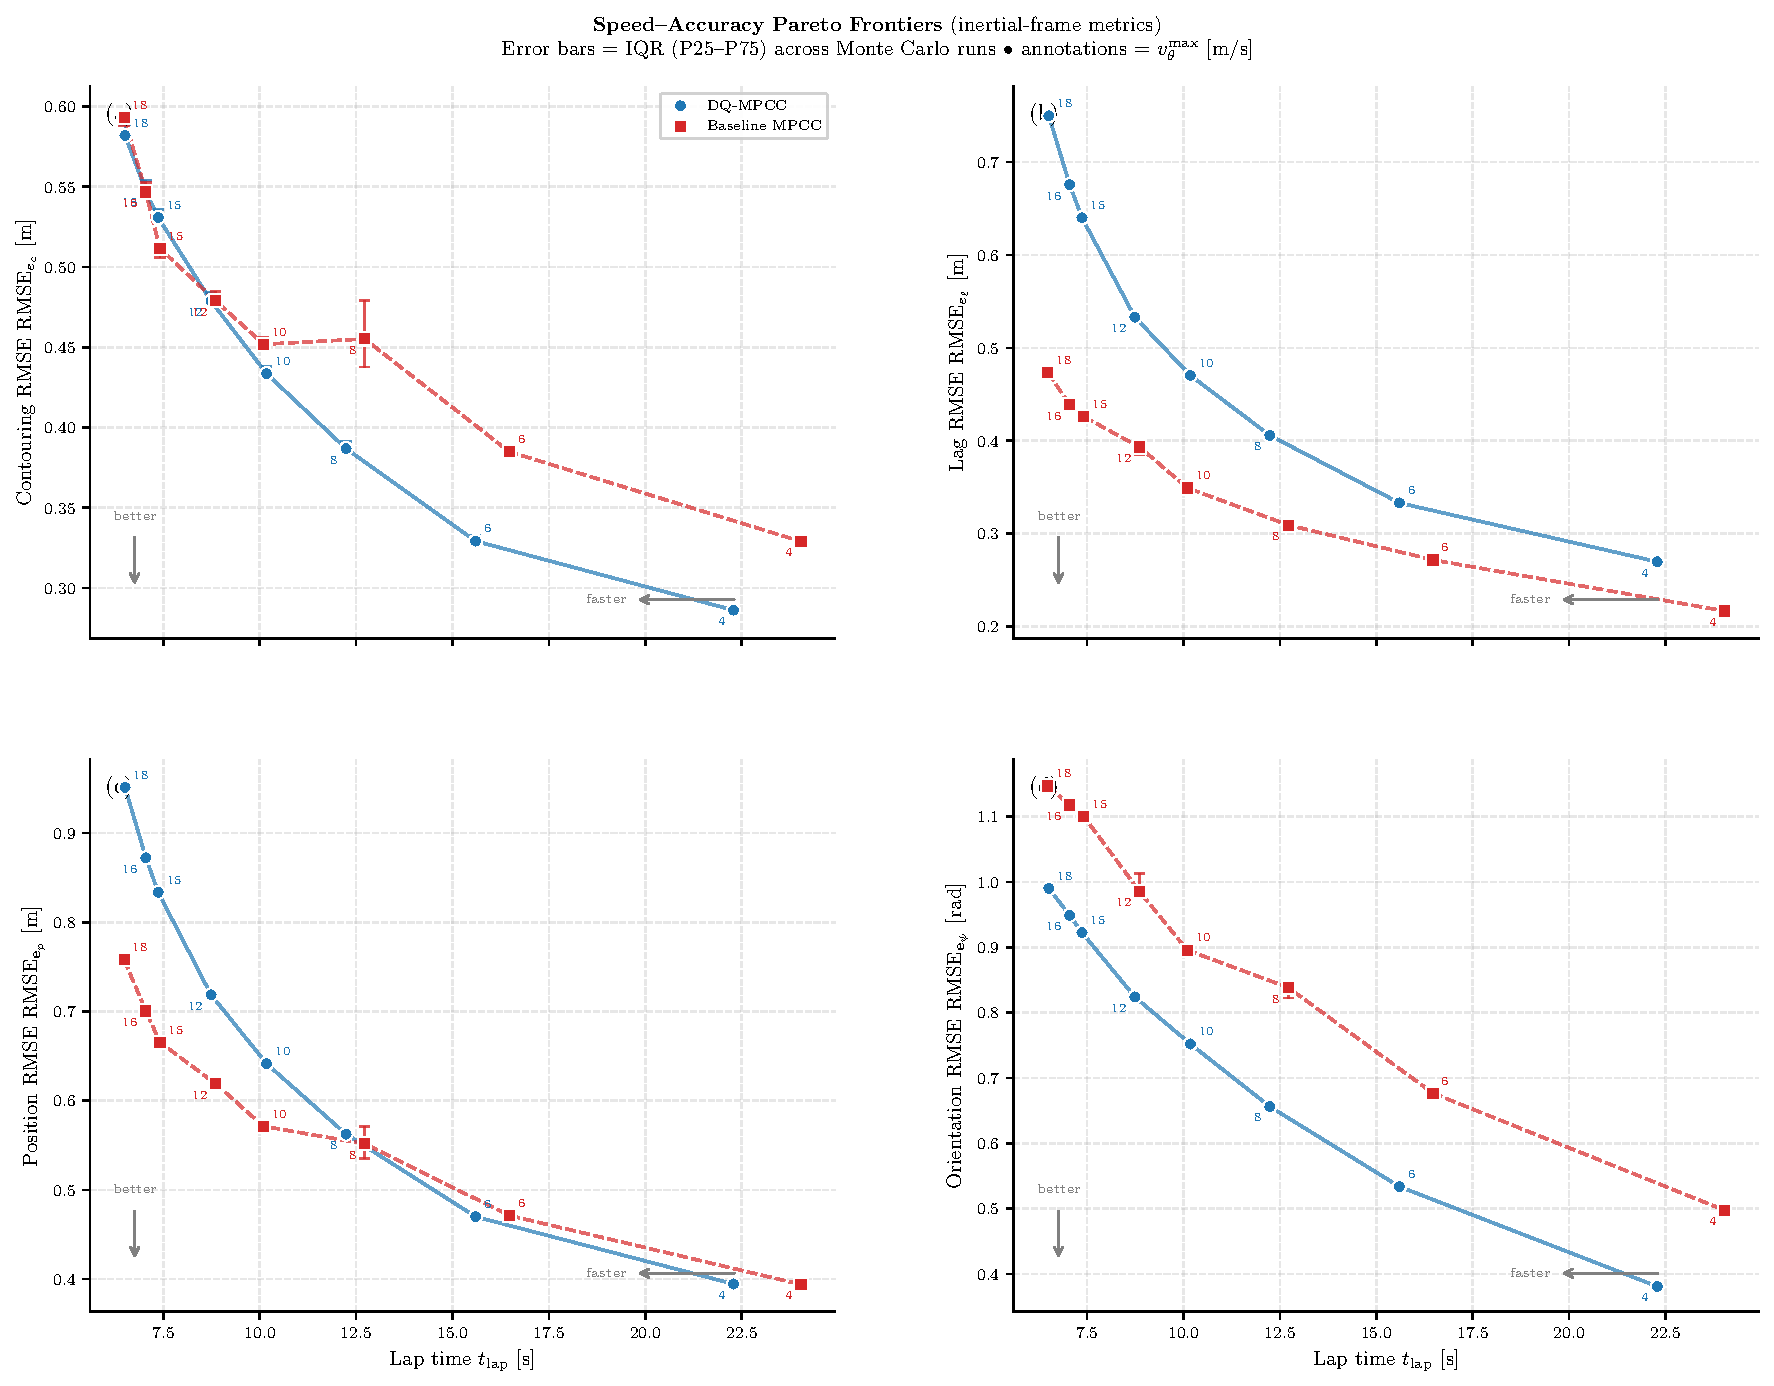
\includegraphics[width=\columnwidth]{fig_pareto_quad.pdf}
    \caption{Speed--accuracy Pareto frontiers for the DQ-MPCC and
Baseline MPCC across 6 progress velocities.
Each point is the median over 5 Monte~Carlo runs;
    error bars denote the interquartile range (P25--P75).
    (a)~Contouring RMSE, (b)~Lag RMSE, (c)~Position RMSE,
    (d)~Orientation RMSE, all vs.\ lap time.
    Annotations indicate $v_\theta^{\max}$ [m/s].}
    \label{fig:pareto_quad}
    \end{figure}

    %% ─────────────────────────────────────────────────────────────────────
    %%  FIGURE ANALYSIS
    %% ─────────────────────────────────────────────────────────────────────

    Fig.~\ref{fig:pareto_quad} presents the speed--accuracy Pareto frontiers
    for both controllers.
    %
    In panel~(a), the Baseline MPCC yields lower contouring RMSE over low and
    medium speeds, whereas the DQ-MPCC becomes superior over part of the tested sweep.
    This indicates that the $\mathrm{SE}(3)$ formulation does not dominate the
    full sweep uniformly, but it becomes increasingly competitive as the
    commanded progress rises.
    %
    Panel~(b) shows a similar trend for lag RMSE: the Baseline is better over
    most of the sweep, while the DQ-MPCC becomes better over part of the tested sweep.
    Hence the DQ formulation does not simply trade contouring against larger
    tangential delay at the top end; instead, both translational components
    improve jointly in the highest-speed regime.
    %
    Panel~(c) combines both components via~\eqref{eq:decomposition}. The total
    position RMSE follows the same pattern, with DQ-MPCC becoming superior over part of the tested sweep,
    while the Baseline remains preferable over the lower and mid-speed region.
    %
    Finally, panel~(d) shows that the Baseline MPCC keeps lower orientation error across the full sweep. Therefore, the
    high-speed translational advantage of DQ-MPCC should not be interpreted as
    a uniform pose-level dominance.

    %% ─────────────────────────────────────────────────────────────────────
    %%  ANALYSIS  (all numbers auto-generated)
    %% ─────────────────────────────────────────────────────────────────────

    \subsubsection{Contouring vs.\ Lag Decomposition}

    Table~\ref{tab:velocity_sweep_full} shows that DQ-MPCC is better on average in contouring RMSE, DQ-MPCC is better on average in lag RMSE, DQ-MPCC is better on average in position RMSE, while baseline mpcc is better on average in orientation rmse.
    The corresponding average deltas for DQ relative to the Baseline are
    $e_c=-2.4\%$, $e_\ell=-2.6\%$, $e_p=-2.5\%$, and $e_\psi=+12.8\%$.
    However, the sign reversal in the high-speed region is important:
    DQ-MPCC first becomes better in contouring at $4$~m/s, and
    its strongest high-speed gains appear at $24$~m/s for position
    ($-6.8\%$) and at $24$~m/s for contouring
    ($-7.0\%$).
    At the same time, DQ-MPCC is consistently faster in lap time across the
    sweep (average $\Delta t_\mathrm{lap}=-2.1\%$),
    so the average tracking deficit does not come from moving more slowly.
    The decomposition in Table~\ref{tab:decomposition} explains this asymmetry:
    the Baseline is \emph{contouring-dominated}
    ($49$--$53\%$ of $\|e_p\|^2$ comes from $e_c$,
    $e_\ell/e_c < 1$ at all speeds),
    while the DQ-MPCC transitions from near parity
    ($53$/$\ 47$\%
    at $4$~m/s) to \emph{lag-dominated}
    ($49$/$\ 51$\%,
    $e_\ell/e_c = 1.03$ at $24$~m/s).
    %
    The root cause is structural: the DQ-MPCC's $\mathrm{SE}(3)$ logarithmic
    error map $\boldsymbol{\rho} = \mathbf{J}_l(\boldsymbol{\varphi})^{-1}
    \mathbf{R}_d^\top \Delta\mathbf{p}$ couples position and orientation,
    while the Baseline penalises $e_c$ and $e_\ell$ as decoupled terms. The
    present results suggest that the decoupled structure is advantageous in the
    low- and mid-speed regime, whereas the coupled DQ formulation becomes more
    competitive, and eventually superior in translational tracking, once the
    demanded progress enters the highest-speed regime.

